\documentclass[11pt,a4paper]{article}

% --- Packages ---
\usepackage[utf8]{inputenc}
\DeclareUnicodeCharacter{00A0}{~}
\usepackage[margin=1in]{geometry}
\usepackage{amsmath,amssymb}
\usepackage{booktabs}
\usepackage{tabularx}
\usepackage{ragged2e}
\usepackage{listings}
\usepackage{xcolor}
\usepackage{float}
\usepackage{fancyhdr}
\usepackage{tikz}
\usetikzlibrary{shapes,arrows.meta,positioning,decorations.pathreplacing,calc,backgrounds,plotmarks}
\usepackage{hyperref}

% Prevent LaTeX from stretching vertical spaces when floats move
\raggedbottom

% --- Hyperref Setup ---
\hypersetup{
    colorlinks=true,
    linkcolor=blue!70!black,
    citecolor=blue!70!black,
    urlcolor=blue!70!black
}

% --- Code Listing Styling ---
\definecolor{codegreen}{rgb}{0,0.6,0}
\definecolor{codegray}{rgb}{0.45,0.45,0.45}
\definecolor{codepurple}{rgb}{0.58,0,0.82}
\definecolor{backcolour}{rgb}{0.96,0.97,0.98}

\lstdefinestyle{cstyle}{
    language=C,
    morekeywords={uint8_t,uint16_t,uint32_t,size_t,PreparedFrame,EthernetFrame},
    backgroundcolor=\color{backcolour},   
    commentstyle=\color{codegreen}\itshape,
    keywordstyle=\color{blue}\bfseries,
    numberstyle=\tiny\color{codegray},
    stringstyle=\color{codepurple},
    basicstyle=\ttfamily\footnotesize,
    breakatwhitespace=false,         
    breaklines=true,                 
    captionpos=b,                    
    keepspaces=true,                 
    numbers=left,                    
    numbersep=6pt,                  
    showspaces=false,                
    showstringspaces=false,
    showtabs=false,                  
    tabsize=4,
    frame=single,
    rulecolor=\color{black!20},
    columns=flexible
}

\lstdefinestyle{hexstyle}{
    backgroundcolor=\color{backcolour},
    basicstyle=\ttfamily\footnotesize,
    columns=flexible,
    numbers=none,
    frame=single,
    rulecolor=\color{black!20},
    breaklines=true,
    keepspaces=true,
    aboveskip=6pt,
    belowskip=6pt
}

\lstset{style=cstyle}

% --- Header and Footer ---
\pagestyle{fancy}
\fancyhf{}
\setlength{\headheight}{14.5pt}
\addtolength{\topmargin}{-2.5pt}
\rhead{Computer Networks Lab: Assignment 2}
\lhead{Flow Control Mechanisms in Data Link Layer}
\cfoot{Page \thepage}

\begin{document}

% =========================================================================
% COVER / TITLE PAGE
% =========================================================================
\hypersetup{pageanchor=false}
\begin{titlepage}
    \centering
    \vspace*{1.5cm}
    
    {\Large \textbf{JADAVPUR UNIVERSITY}}\\[0.3cm]
    {\large DEPARTMENT OF COMPUTER SCIENCE AND ENGINEERING}\\[2.0cm]
    
    \rule{\linewidth}{1.2pt}\\[0.4cm]
    {\huge \textbf{Assignment 2 Report}}\\[0.3cm]
    {\LARGE \textbf{Design and Implementation of Flow Control Mechanisms in Data Link Layer}}\\[0.3cm]
    {\large \textit{Empirical Evaluation of Stop-and-Wait, Go-Back-N ARQ, and Selective Repeat ARQ Protocols over a Simulated Socket Network}}\\[0.4cm]
    \rule{\linewidth}{1.2pt}\\[2.2cm]
    
    \begin{flushleft}
        \large
        \textbf{Course:} Computer Networks Laboratory (BCSE-III)\\[0.2cm]
        \textbf{Student Name:} Mandeep Shaw\\[0.2cm]
        \textbf{Section:} A1\\[0.2cm]
        \textbf{Roll Number:} 302510501002\\[0.2cm]
        \textbf{Assignment:} Assignment 2 (Flow Control: Stop-and-Wait, Go-Back-N ARQ, Selective Repeat ARQ)\\[0.2cm]
        \textbf{Date of Submission:} October 2026
    \end{flushleft}
    
    \vfill
    {\small Faculty of Engineering and Technology $\bullet$ Jadavpur University, Kolkata, India}
\end{titlepage}
\hypersetup{pageanchor=true}

% =========================================================================
% TABLE OF CONTENTS
% =========================================================================
\tableofcontents
\newpage

% =========================================================================
% SECTION 1: INTRODUCTION AND OBJECTIVES
% =========================================================================
\section{Introduction and Objectives}

In computer network architectures, physical transmission channels are inherently unreliable and subject to bandwidth limitations, propagation delays, and burst noise. If a sender transmits data at a rate exceeding the processing or buffer capacity of the receiver, intermediate buffers overflow, causing packet loss. Similarly, unmitigated channel errors lead to corrupted payloads. To ensure reliable, in-order, and rate-regulated delivery of data, the Data Link Layer (specifically the Logical Link Control sublayer) implements \textbf{Flow Control} and \textbf{Automatic Repeat reQuest (ARQ)} mechanisms.

The primary objective of this assignment is to design, implement, and benchmark the three foundational flow control protocols in C over a simulated client-server network:
\begin{enumerate}
    \item \textbf{Stop-and-Wait Protocol (Noiseless and Noisy ARQ):} Transmission of a single frame per time slot with receiver acknowledgment, idle sender waiting time, and timeout-based retransmission.
    \item \textbf{Go-Back-N (GBN) ARQ Scheme:} Pipelined sliding-window transmission with sender window size \(N\) and receiver window size \(1\), utilizing cumulative acknowledgments and full-window retransmission on frame loss.
    \item \textbf{Selective Repeat (SR) ARQ Protocol:} Full duplex sliding-window transmission with window size \(N\) at both sender and receiver, utilizing independent acknowledgments, receiver buffering for out-of-order packets, and targeted retransmissions of lost frames.
    \item \textbf{Socket-Based Network Simulation:} Construction of a modular client-server socket pipeline over TCP/IP loopback, integrating 65-byte IEEE 802.3-style Ethernet framing, 32-bit CRC error detection from Assignment 1, and stochastic channel impairments (bit corruption, packet loss, and transmission delays).
    \item \textbf{Empirical Performance Profiling:} Exhaustive benchmarking across test scenarios measuring round-trip times (\(RTT\)), protocol efficiency under error-free conditions, and resilience across error/loss probabilities ranging from \(p = 0.10\) to \(p = 0.50\).
\end{enumerate}

% =========================================================================
% SECTION 2: THEORETICAL PRINCIPLES OF FLOW CONTROL
% =========================================================================
\section{Theoretical Principles of Flow Control}

Flow control regulates the rate of data transmission between communicating entities so that a fast sender cannot overwhelm a slow receiver. Error control provides the complementary mechanism to detect and retransmit corrupted or missing frames. Together, they form ARQ protocols.

\subsection{Channel Propagation Delay and Bandwidth-Delay Product}

Let \(L_f\) be the frame length in bits, \(B\) be the channel bandwidth in bits per second, and \(d\) be the physical distance between sender and receiver with signal propagation velocity \(v\). The key timing components are:
\begin{align}
    \text{Frame Transmission Time: } & T_{\text{tx}} = \frac{L_f}{B} \\
    \text{Channel Propagation Time: } & T_{\text{prop}} = \frac{d}{v} \\
    \text{ACK Transmission Time: } & T_{\text{ack}} = \frac{L_{\text{ack}}}{B}
\end{align}
The normalized channel delay parameter \(a\) is defined as the ratio of propagation delay to transmission delay:
\begin{equation}
    a = \frac{T_{\text{prop}}}{T_{\text{tx}}}
\end{equation}
When \(a \gg 1\) (such as in satellite or high-speed wide-area links), the channel capacity is dominated by propagation delay, making simple stop-and-wait approaches grossly inefficient.

\subsection{Stop-and-Wait Flow Control and ARQ}

In the classic \textbf{Stop-and-Wait} protocol:
\begin{enumerate}
    \item The sender transmits a single frame and starts a retransmission timer.
    \item The sender enters an idle waiting state, doing no useful work until an acknowledgment (ACK) frame is received.
    \item The total time required to deliver one frame and receive its ACK is the Round-Trip Time (\(RTT\)):
    \begin{equation}
        T_{\text{total}} = T_{\text{tx}} + 2 \cdot T_{\text{prop}} + T_{\text{proc}} + T_{\text{ack}}
    \end{equation}
\end{enumerate}
Under ideal conditions where \(T_{\text{proc}}\) and \(T_{\text{ack}}\) are negligible, the maximum channel utilization (efficiency \(\eta\)) is:
\begin{equation}
    \eta_{\text{SW}} = \frac{T_{\text{tx}}}{T_{\text{tx}} + 2 T_{\text{prop}}} = \frac{1}{1 + 2a}
\end{equation}
In a \textbf{Noiseless Channel}, frame loss does not occur. However, if an error does occur and the receiver discards the corrupted frame without responding, a protocol without a timer enters an \textbf{indefinite deadlock}.

In \textbf{Stop-and-Wait ARQ}, a timer is associated with the transmitted frame. If an ACK does not arrive within a specified timeout threshold (\(T_{\text{out}} \ge RTT\)), the sender times out and retransmits the frame. To distinguish between new frames and duplicate retransmissions, a 1-bit sequence number (\(0\) and \(1\)) is embedded in the frame header. If frame error probability is \(p\), the expected number of transmissions per frame is \(\frac{1}{1 - p}\), yielding an effective efficiency:
\begin{equation}
    \eta_{\text{SW-ARQ}} = \frac{1 - p}{1 + 2a}
\end{equation}

\subsection{Go-Back-N (GBN) ARQ Protocol}

To eliminate the idle waiting time of Stop-and-Wait, \textbf{pipelined} protocols allow the sender to transmit multiple frames before receiving an acknowledgment.

In \textbf{Go-Back-N ARQ}:
\begin{itemize}
    \item \textbf{Sender Window (\(W_s = N\)):} The sender can transmit up to \(N\) consecutive unacknowledged frames.
    \item \textbf{Receiver Window (\(W_r = 1\)):} The receiver accepts only frames that arrive strictly \textbf{in order}.
    \item \textbf{Cumulative Acknowledgments:} An ACK with sequence number \(i\) confirms receipt of frame \(i\) and all preceding frames (\(0, 1, \dots, i-1\)).
    \item \textbf{Error Handling:} If frame \(k\) is lost or corrupted, the receiver discards frame \(k\) and silently discards all subsequent out-of-order frames (\(k+1, k+2, \dots\)), even if they arrive undamaged. When the sender's timer for frame \(k\) expires, the sender must ``go back \(N\)'' and retransmit all unacknowledged frames currently in the pipeline (\([k, \dots, \text{nextSeq}-1]\)).
\end{itemize}
The maximum theoretical efficiency in an error-free channel is:
\begin{equation}
    \eta_{\text{GBN}} = \min\left(1, \; \frac{N}{1 + 2a}\right)
\end{equation}
However, under noisy channels with frame loss probability \(p\), GBN suffers a severe retransmission multiplication penalty, as every single loss forces the retransmission of an entire window of \(N\) frames:
\begin{equation}
    \eta_{\text{GBN}}(p) = \frac{1 - p}{1 + (N - 1)p} \cdot \min\left(1, \; \frac{N}{1 + 2a}\right)
\end{equation}

\subsection{Selective Repeat (SR) ARQ Protocol}

\textbf{Selective Repeat ARQ} optimizes bandwidth utilization by avoiding unnecessary retransmissions of correctly received frames:
\begin{itemize}
    \item \textbf{Sender Window (\(W_s = N\)):} The sender maintains a window of \(N\) frames.
    \item \textbf{Receiver Window (\(W_r = N\)):} The receiver maintains a buffer of size \(N\), allowing it to accept and store out-of-order frames within the valid window range.
    \item \textbf{Independent Acknowledgments:} Each frame is acknowledged individually. Receiving an ACK for frame \(k+1\) does not acknowledge frame \(k\).
    \item \textbf{Selective Retransmission:} When a timeout occurs, the sender retransmits \textbf{only} the specific unacknowledged frame(s), rather than the entire window.
    \item \textbf{In-Order Delivery:} The receiver delivers buffered frames to the application layer in strictly sorted sequence once missing intermediate frames arrive.
\end{itemize}
The effective efficiency of Selective Repeat under frame error probability \(p\) is:
\begin{equation}
    \eta_{\text{SR}}(p) = (1 - p) \cdot \min\left(1, \; \frac{N}{1 + 2a}\right)
\end{equation}
Unlike Go-Back-N, the efficiency of Selective Repeat does not suffer from window-multiplication degradation under noisy channels.

\subsection{Sequence Number Space Constraint}

To prevent sequence number ambiguity caused by delayed duplicates, the sequence number space \(M = 2^m\) (where \(m\) is the bit width of the sequence number field) must satisfy:
\begin{equation}
    W_s + W_r \le 2^m
\end{equation}
For Go-Back-N (\(W_r = 1\)), the maximum sender window is \(W_s \le 2^m - 1\). For Selective Repeat (\(W_s = W_r = N\)), the window size is strictly bounded by:
\begin{equation}
    N \le 2^{m-1} = \frac{2^m}{2}
\end{equation}
In our implementation, sequence numbers are represented as an 8-bit unsigned integer (\(m = 8\), range \(0..255\)), easily satisfying \(W_s \le 64 < 128\).

% =========================================================================
% SECTION 3: SYSTEM ARCHITECTURE AND DESIGN
% =========================================================================
\section{System Architecture and Procedural Design}

\subsection{System Overview and Procedural Organization}

The system is organized into a modular client-server socket pipeline operating over TCP/IP loopback (\texttt{127.0.0.1:5000}). Figure~\ref{fig:arch_diagram} illustrates the procedural organization, depicting the interaction between the sender, simulated physical channel, and receiver.

\begin{figure}[H]
    \centering
    \resizebox{\textwidth}{!}{%
    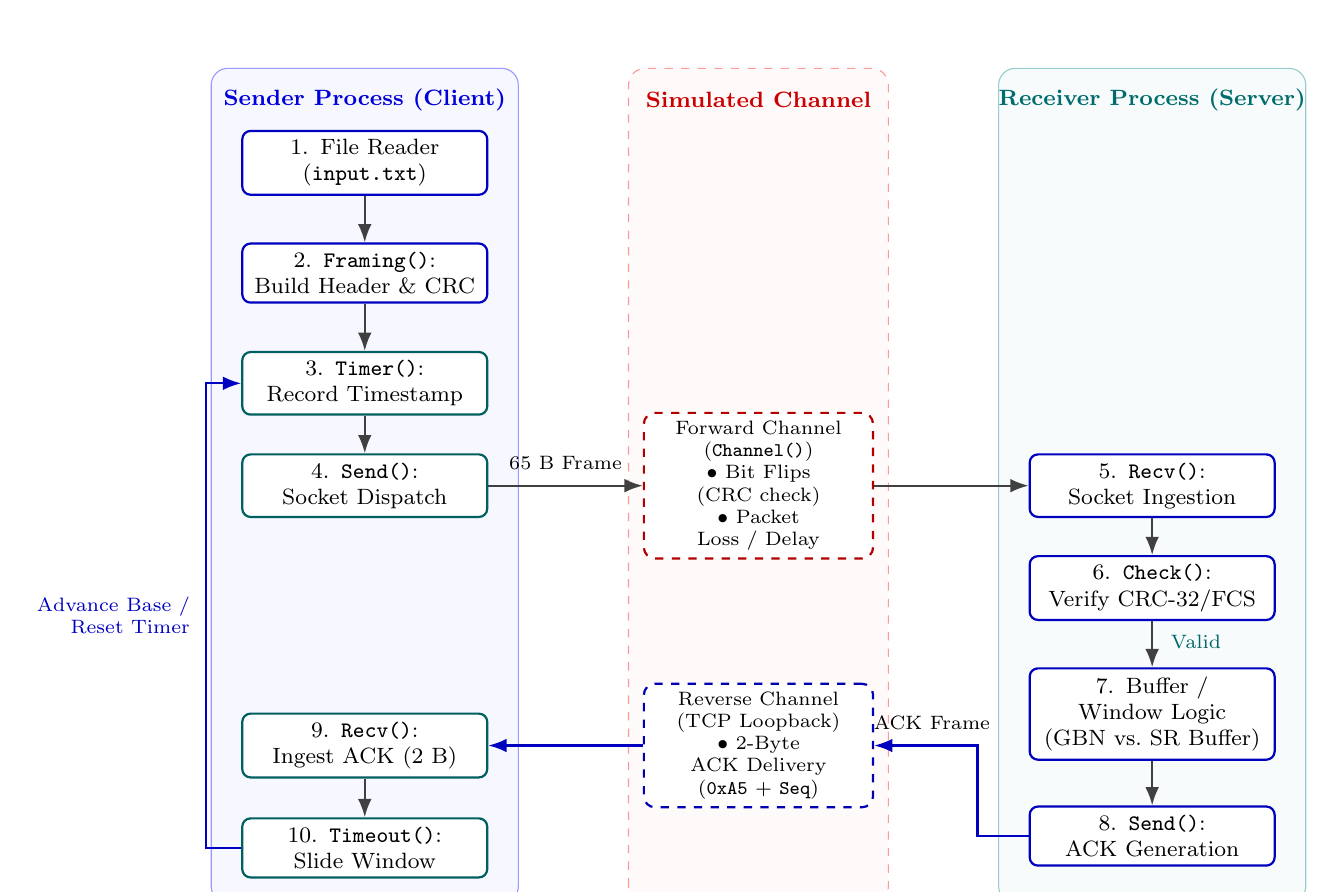
\begin{tikzpicture}[
        font=\footnotesize,
        >=Latex,
        block/.style={rectangle, draw=blue!75!black, fill=white, thick, rounded corners=3pt, minimum height=0.75cm, text width=2.9cm, align=center, inner sep=3pt},
        proc/.style={rectangle, draw=teal!75!black, fill=white, thick, rounded corners=3pt, minimum height=0.75cm, text width=2.9cm, align=center, inner sep=3pt},
        chan/.style={rectangle, draw=red!70!black, fill=white, thick, dashed, rounded corners=4pt, minimum height=1.25cm, text width=2.7cm, align=center, font=\scriptsize, inner sep=3pt},
        arrow/.style={->, thick, draw=black!75},
        retarrow/.style={->, thick, draw=blue!75!black}
    ]
        % ==================== BACKGROUND CONTAINERS ====================
        \begin{scope}[on background layer]
            \draw[draw=blue!40, fill=blue!3, rounded corners=6pt] (-0.25, -4.55) rectangle (3.65, 6.05);
            \draw[draw=red!40, fill=red!2, dashed, rounded corners=6pt] (5.05, -4.55) rectangle (8.35, 6.05);
            \draw[draw=teal!40, fill=teal!3, rounded corners=6pt] (9.75, -4.55) rectangle (13.65, 6.05);
        \end{scope}

        % Container Header Labels
        \node[font=\bfseries\footnotesize, text=blue!85!black] at (1.7, 5.65) {Sender Process (Client)};
        \node[font=\bfseries\footnotesize, text=red!80!black]  at (6.7, 5.65) {Simulated Channel};
        \node[font=\bfseries\footnotesize, text=teal!85!black] at (11.7, 5.65) {Receiver Process (Server)};

        % ==================== SENDER (x = 1.7) ====================
        \node[block] (input) at (1.7, 4.85) {1. File Reader\\(\texttt{input.txt})};
        \node[block] (frame) at (1.7, 3.45) {2. \texttt{Framing()}:\\Build Header \& CRC};
        \node[proc]  (timer) at (1.7, 2.05) {3. \texttt{Timer()}:\\Record Timestamp};
        \node[proc]  (send)  at (1.7, 0.75) {4. \texttt{Send()}:\\Socket Dispatch};

        \node[proc]  (srecv) at (1.7, -2.55) {9. \texttt{Recv()}:\\Ingest ACK (2 B)};
        \node[proc]  (tout)  at (1.7, -3.85) {10. \texttt{Timeout()}:\\Slide Window};

        % ==================== CHANNEL (x = 6.7) ====================
        \node[chan] (fwd_chan) at (6.7, 0.75) {Forward Channel\\(\texttt{Channel()})\\\(\bullet\) Bit Flips (CRC check)\\\(\bullet\) Packet Loss / Delay};
        \node[chan, draw=blue!70!black] (rev_chan) at (6.7, -2.55) {Reverse Channel\\(TCP Loopback)\\\(\bullet\) 2-Byte ACK Delivery\\(\texttt{0xA5} + \texttt{Seq})};

        % ==================== RECEIVER (x = 11.7) ====================
        \node[block] (rrecv)  at (11.7, 0.75)  {5. \texttt{Recv()}:\\Socket Ingestion};
        \node[block] (check)  at (11.7, -0.55) {6. \texttt{Check()}:\\Verify CRC-32/FCS};
        \node[block] (buf)    at (11.7, -2.15) {7. Buffer / Window Logic\\(GBN vs.\ SR Buffer)};
        \node[block] (ack)    at (11.7, -3.70) {8. \texttt{Send()}:\\ACK Generation};

        % ==================== FORWARD PATH ====================
        \draw[arrow] (input) -- (frame);
        \draw[arrow] (frame) -- (timer);
        \draw[arrow] (timer) -- (send);
        \draw[arrow] (send) -- node[above=2pt, font=\scriptsize] {65 B Frame} (fwd_chan);
        \draw[arrow] (fwd_chan) -- (rrecv);
        \draw[arrow] (rrecv) -- (check);
        \draw[arrow] (check) -- node[pos=0.45, right=3pt, font=\scriptsize, text=teal!80!black] {Valid} (buf);
        \draw[arrow] (buf) -- (ack);

        % ==================== REVERSE / ACK PATH ====================
        \draw[retarrow] (ack.west) -- ++(-0.65, 0) |- node[pos=0.72, above=2pt, font=\scriptsize] {ACK Frame} (rev_chan.east);
        \draw[retarrow] (rev_chan) -- (srecv);
        \draw[arrow] (srecv) -- (tout);

        % Feedback to Window / Timer
        \draw[arrow, blue!75!black] (tout.west) -- ++(-0.45,0) |-
            node[pos=0.25, left=2pt, font=\scriptsize, align=right] {Advance Base /\\Reset Timer}
            (timer.west);

    \end{tikzpicture}%
    }
    \caption{Procedural organization and end-to-end data link flow control architecture.}
    \label{fig:arch_diagram}
\end{figure}

\subsection{Frame Structure and In-Memory Layout}

To conform strictly to the assignment specifications, the data frame consists of a 15-byte header, a 46-byte payload, and a 4-byte Frame Check Sequence (FCS) trailer, totaling 65 bytes.

\begin{figure}[H]
    \centering
    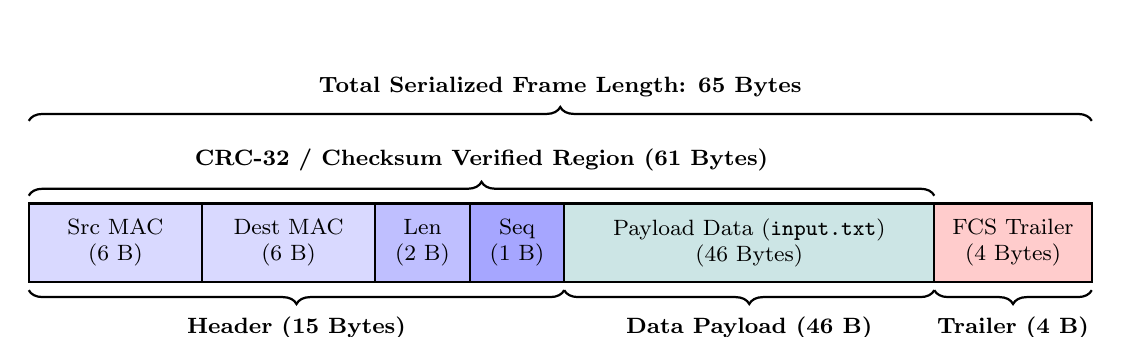
\begin{tikzpicture}[font=\footnotesize]
        % Header blocks
        \draw[fill=blue!15, thick] (0,0) rectangle (2.2, 1.0) node[pos=0.5, align=center] {Src MAC\\(6 B)};
        \draw[fill=blue!15, thick] (2.2,0) rectangle (4.4, 1.0) node[pos=0.5, align=center] {Dest MAC\\(6 B)};
        \draw[fill=blue!25, thick] (4.4,0) rectangle (5.6, 1.0) node[pos=0.5, align=center] {Len\\(2 B)};
        \draw[fill=blue!35, thick] (5.6,0) rectangle (6.8, 1.0) node[pos=0.5, align=center] {Seq\\(1 B)};

        % Payload block
        \draw[fill=teal!20, thick] (6.8,0) rectangle (11.5, 1.0) node[pos=0.5, align=center] {Payload Data (\texttt{input.txt})\\(46 Bytes)};

        % Trailer block
        \draw[fill=red!20, thick] (11.5,0) rectangle (13.5, 1.0) node[pos=0.5, align=center] {FCS Trailer\\(4 Bytes)};

        % Braces and labels
        \draw[decorate, decoration={brace, mirror, amplitude=5pt}, thick] (0,-0.1) -- (6.8,-0.1)
            node[pos=0.5, below=6pt] {\textbf{Header (15 Bytes)}};
        \draw[decorate, decoration={brace, mirror, amplitude=5pt}, thick] (6.8,-0.1) -- (11.5,-0.1)
            node[pos=0.5, below=6pt] {\textbf{Data Payload (46 B)}};
        \draw[decorate, decoration={brace, mirror, amplitude=5pt}, thick] (11.5,-0.1) -- (13.5,-0.1)
            node[pos=0.5, below=6pt] {\textbf{Trailer (4 B)}};
        \draw[decorate, decoration={brace, amplitude=5pt}, thick] (0,1.1) -- (11.5,1.1)
            node[pos=0.5, above=5pt] {\textbf{CRC-32 / Checksum Verified Region (61 Bytes)}};
        \draw[decorate, decoration={brace, amplitude=5pt}, thick] (0,2.05) -- (13.5,2.05)
            node[pos=0.5, above=5pt] {\textbf{Total Serialized Frame Length: 65 Bytes}};
    \end{tikzpicture}
    \caption{In-memory layout and serialization structure of the Data Link Frame.}
    \label{fig:frame_layout}
\end{figure}

The acknowledgment frame is compact (2 bytes):
\begin{equation}
    \text{ACK Frame} = \big[\, \texttt{Marker (0xA5)} \; (1\text{ Byte}) \;\mid\; \texttt{Ack Sequence Number} \; (1\text{ Byte}) \,\big]
\end{equation}

\subsection{Input and Output Formats}

\begin{itemize}
    \item \textbf{Input Format:} The sender reads ASCII text from an input file (\texttt{input.txt}). Payloads are chunked into 46-byte blocks. Any partial terminal block is zero-padded up to 46 bytes.
    \item \textbf{Output Format:} Both sender and receiver output verbose transmission status logs to \texttt{stdout}:
    \begin{itemize}
        \item Frame sequence number, MAC addresses, payload length.
        \item Hexadecimal byte dumps and ASCII representations of transmitted and received payloads.
        \item Computed and received FCS values (CRC-32 or Checksum).
        \item Channel outcome: \texttt{NO ERROR}, \texttt{ERROR INJECTED}, or \texttt{TIMEOUT}.
        \item Sliding window status, cumulative/selective ACK reception, and window advance notifications.
    \end{itemize}
\end{itemize}

% =========================================================================
% SECTION 4: IMPLEMENTATION DETAILS
% =========================================================================
\section{Implementation Details}

\subsection{Key Methods and Interfaces}

Table~\ref{tab:methods} summarizes the programmatic methods implemented across the sender and receiver modules.

\begin{table}[htbp]
    \centering
    \small
    \begin{tabularx}{\textwidth}{ll>{\RaggedRight\arraybackslash}X}
        \toprule
        \textbf{Entity} & \textbf{Method Name} & \textbf{Functional Description} \\
        \midrule
        \textbf{Sender} & \texttt{Framing()} & Constructs 65-byte frame from input payload, attaches MAC addresses, sets sequence number, and appends FCS trailer. \\
        & \texttt{Channel()} & Simulates physical channel impairments: injects bit flips (single, double, odd, burst) and drops/delays frames. \\
        & \texttt{Send()} & Serializes frame and transmits it over socket; triggers retransmission if an ACK is not received. \\
        & \texttt{Timer()} & Tracks frame dispatch timestamp; enforces the 1500 ms socket timeout. \\
        & \texttt{Timeout()} & Calculates round-trip time (\(RTT\)) for the frame and computes adaptive timeout thresholds. \\
        & \texttt{Recv()} & Listens for incoming 2-byte ACK frames from receiver socket. \\
        \midrule
        \textbf{Receiver} & \texttt{Recv()} & Receives 3-byte control prefix and 65-byte packed data frame from TCP stream. \\
        & \texttt{Check()} & Computes CRC-32/Checksum across 61-byte verified region; discards frame if verification fails. \\
        & \texttt{Send()} & Prepares and transmits 2-byte ACK frame (\texttt{0xA5} + \texttt{seqNo}) back to sender. \\
        \bottomrule
    \end{tabularx}
    \caption{Functional mapping of sender and receiver methods.}
    \label{tab:methods}
\end{table}

\subsection{Core Code Snippets}

Listing~\ref{lst:gbn} illustrates the transmission and cumulative ACK processing loop for Go-Back-N ARQ from \texttt{sender.c}:

\begin{lstlisting}[language=C, caption={Go-Back-N sliding window and timeout retransmission loop (sender.c).}, label={lst:gbn}]
while (base < frameCount) {
    /* Transmit all new frames within the current window */
    while (nextSeq < frameCount && nextSeq < base + windowSize) {
        PreparedFrame *pf = &frames[nextSeq];
        transmitFrameOnce(sock, pf, channelType, 0, MAX_RETRIES);
        nextSeq++;
    }

    /* Wait for cumulative ACK */
    if (receiveACK(sock, ack) && ack[0] == ACK_MARKER) {
        uint8_t ackSeq = ack[1];
        int matched = -1;
        for (int k = base; k < nextSeq; k++) {
            if (frames[k].frame.sequenceNumber == ackSeq) {
                matched = k;
                break;
            }
        }
        if (matched >= base) {
            printf("Cumulative ACK %u received (advances base from %d to %d)\n",
                   ackSeq, base, matched + 1);
            base = matched + 1;
            retries = 0;
        }
    } else {
        /* Timeout on window base: retransmit entire window */
        retries++;
        printf("Timeout on sequence %u. Retransmitting window [%d..%d]\n",
               frames[base].frame.sequenceNumber, base, nextSeq - 1);
        for (int k = base; k < nextSeq; k++) {
            transmitFrameOnce(sock, &frames[k], channelType, retries, MAX_RETRIES);
        }
    }
}
\end{lstlisting}

Listing~\ref{lst:sr} demonstrates out-of-order buffering, independent ACK dispatch, and ordered delivery in Selective Repeat ARQ from \texttt{receiver.c}:

\begin{lstlisting}[language=C, caption={Selective Repeat out-of-order buffering and sorted frame delivery (receiver.c).}, label={lst:sr}]
uint8_t dist = (uint8_t)(frame.sequenceNumber - expectedSequence);
if (dist < (uint8_t)windowSize) {
    if (!srBuffer[frame.sequenceNumber].occupied) {
        srBuffer[frame.sequenceNumber].occupied = 1;
        srBuffer[frame.sequenceNumber].frame = frame;
        printf("Out-of-order frame %u buffered in window\n", frame.sequenceNumber);
    }
    /* Send independent ACK for received frame */
    sendACK(clientSocket, frame.sequenceNumber);

    /* Deliver all consecutive in-order buffered frames */
    while (srBuffer[expectedSequence].occupied) {
        EthernetFrame *accepted = &srBuffer[expectedSequence].frame;
        printf("Delivering sorted frame sequence %u to application\n",
               accepted->sequenceNumber);
        srBuffer[expectedSequence].occupied = 0;
        expectedSequence = (uint8_t)(expectedSequence + 1);
    }
}
\end{lstlisting}

% =========================================================================
% SECTION 5: TEST CASES AND EXPERIMENTAL METHODOLOGY
% =========================================================================
\section{Test Cases and Experimental Methodology}

To rigorously evaluate the flow control implementations as specified in the assignment guidelines, four structured test scenarios were executed:

\begin{itemize}
    \item \textbf{Test Case 1: Propagation Delay vs.\ ACK Reception Time (\(RTT\) Dynamics):}
    Evaluates the latency between packet transmission and ACK reception across five payload sizes (\(46, 128, 512, 1024, 1500\) bytes) and four propagation delays (\(5.0, 10.0, 20.0, 50.0\) ms) over a simulated 10 Mbps channel. Verifies dynamic timeout threshold computation:
    \begin{equation}
        T_{\text{out}} = 2 \cdot RTT + 5.0\text{ ms}
    \end{equation}

    \item \textbf{Test Case 2: Protocol Efficiency in an Error-Free (Noiseless) Channel (\(p = 0.0\)):}
    Transmits \(10{,}000\) consecutive frames under perfect channel conditions to measure baseline transmission efficiency (defined empirically as the goodput ratio \(\text{Frames Delivered} / \text{Total Transmitted}\)), transmission count, and average per-frame delivery delay across window sizes \(N \in \{1, 2, 4, 8, 16\}\).

    \item \textbf{Test Case 3: Protocol Efficiency and Retransmissions under Error Probabilities (\(p = 0.10\) to \(0.50\)):}
    Applies independent stochastic corruption and drop probabilities (\(p \in \{0.10, 0.20, 0.30, 0.40, 0.50\}\)) across \(10{,}000\) delivered frames per configuration. Measures empirical transmission efficiency (\(\text{Delivered} / \text{Total Tx}\)), total retransmissions, timeouts, and compares the window-multiplication degradation of Go-Back-N against Selective Repeat.

    \item \textbf{Test Case 4: Live Socket Loopback Execution and Protocol Trace Verification:}
    Executes compiled sender and receiver binaries over TCP loopback (\texttt{127.0.0.1:5000}) using the 276-byte \texttt{input.txt} dataset (6 frames) to observe live framing, corruption detection via CRC-32, timeout triggering, cumulative ACK window advancement, and out-of-order buffer reassembly.
\end{itemize}

% =========================================================================
% SECTION 6: EXPERIMENTAL RESULTS AND EMPIRICAL EVALUATION
% =========================================================================
\section{Experimental Results and Empirical Evaluation}

\subsection{Test Case 1: Propagation Delay vs. ACK Reception Time}

Table~\ref{tab:test1_rtt} summarizes the empirical timing breakdown across varying payload sizes and propagation delays.

\begin{table}[H]
    \centering
    \footnotesize
    \renewcommand{\arraystretch}{0.92}
    \setlength{\tabcolsep}{8pt}
    \begin{tabular}{cccccc}
        \toprule
        \textbf{Payload} & \(\boldsymbol{T_{\text{prop}}}\) & \(\boldsymbol{T_{\text{tx}}}\) \textbf{Frame} & \(\boldsymbol{T_{\text{tx}}}\) \textbf{ACK} & \textbf{Measured} & \textbf{Timeout} \\
        \textbf{(Bytes)} & \textbf{(ms)} & \textbf{(ms)} & \textbf{(ms)} & \textbf{RTT (ms)} & \textbf{Threshold (ms)} \\
        \midrule
        46   & 5.0  & 0.0520 & 0.0016 & 10.104 & 25.207 \\
        46   & 10.0 & 0.0520 & 0.0016 & 20.104 & 45.207 \\
        46   & 20.0 & 0.0520 & 0.0016 & 40.104 & 85.207 \\
        46   & 50.0 & 0.0520 & 0.0016 & 100.104 & 205.207 \\
        \midrule
        128  & 5.0  & 0.1176 & 0.0016 & 10.169 & 25.338 \\
        128  & 10.0 & 0.1176 & 0.0016 & 20.169 & 45.338 \\
        128  & 20.0 & 0.1176 & 0.0016 & 40.169 & 85.338 \\
        128  & 50.0 & 0.1176 & 0.0016 & 100.169 & 205.338 \\
        \midrule
        512  & 5.0  & 0.4248 & 0.0016 & 10.476 & 25.953 \\
        512  & 10.0 & 0.4248 & 0.0016 & 20.476 & 45.953 \\
        512  & 20.0 & 0.4248 & 0.0016 & 40.476 & 85.953 \\
        512  & 50.0 & 0.4248 & 0.0016 & 100.476 & 205.953 \\
        \midrule
        1024 & 5.0  & 0.8344 & 0.0016 & 10.886 & 26.772 \\
        1024 & 10.0 & 0.8344 & 0.0016 & 20.886 & 46.772 \\
        1024 & 20.0 & 0.8344 & 0.0016 & 40.886 & 86.772 \\
        1024 & 50.0 & 0.8344 & 0.0016 & 100.886 & 206.772 \\
        \midrule
        1500 & 5.0  & 1.2152 & 0.0016 & 11.267 & 27.534 \\
        1500 & 10.0 & 1.2152 & 0.0016 & 21.267 & 47.534 \\
        1500 & 20.0 & 1.2152 & 0.0016 & 41.267 & 87.534 \\
        1500 & 50.0 & 1.2152 & 0.0016 & 101.267 & 207.534 \\
        \bottomrule
    \end{tabular}
    \caption{RTT and timeout dynamics across payload sizes and propagation delays (10 Mbps channel).}
    \label{tab:test1_rtt}
\end{table}

\begin{figure}[H]
    \centering
    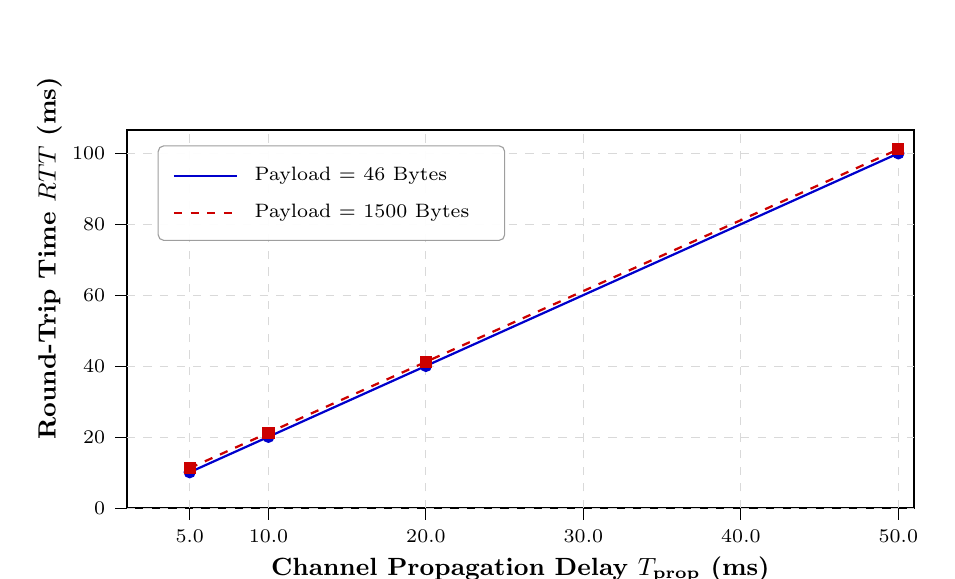
\begin{tikzpicture}[font=\footnotesize]
        % --- GRID & AXIS BOX ---
        \draw[thick] (0.8, 0) rectangle (10.8, 4.8);

        % Horizontal grid lines & Y ticks (0 to 100 ms, scale: 0.9 cm = 20 ms)
        \foreach \y/\val in {0/0, 0.9/20, 1.8/40, 2.7/60, 3.6/80, 4.5/100} {
            \draw[dashed, black!15] (0.8, \y) -- (10.8, \y);
            \draw (0.8, \y) -- (0.65, \y) node[left, font=\scriptsize] {\val};
        }

        % Vertical grid lines & X ticks (scale: 1 cm = 5 ms -> coords 0.8 to 10.8)
        \foreach \x/\val in {1.6/5.0, 2.6/10.0, 4.6/20.0, 6.6/30.0, 8.6/40.0, 10.6/50.0} {
            \draw[dashed, black!15] (\x, 0) -- (\x, 4.8);
            \draw (\x, 0) -- (\x, -0.15) node[below, font=\scriptsize] {\val};
        }

        % Axis Labels
        \node[below=14pt, font=\small\bfseries] at (5.8, 0) {Channel Propagation Delay \(T_{\text{prop}}\) (ms)};
        \node[above=22pt, font=\small\bfseries, rotate=90] at (0.1, 2.4) {Round-Trip Time \(RTT\) (ms)};

        % --- PLOTS ---
        % Payload 46 B
        \draw[thick, blue!80!black, mark=*, mark size=1.8pt] plot coordinates {
            (1.6, 0.455) (2.6, 0.905) (4.6, 1.805) (10.6, 4.505)
        };

        % Payload 1500 B
        \draw[thick, red!80!black, dashed, mark=square*, mark size=1.8pt, mark options={solid}] plot coordinates {
            (1.6, 0.507) (2.6, 0.957) (4.6, 1.857) (10.6, 4.557)
        };

        % --- LEGEND BOX (Top-Left) ---
        \draw[fill=white, draw=black!40, rounded corners=2pt, opacity=0.95] (1.2, 3.4) rectangle (5.6, 4.6);
        \begin{scope}[font=\scriptsize]
            \draw[thick, blue!80!black, mark=*, mark size=1.5pt] (1.4, 4.22) -- (2.2, 4.22);
            \node[right] at (2.3, 4.22) {Payload = 46 Bytes};

            \draw[thick, red!80!black, dashed, mark=square*, mark size=1.5pt, mark options={solid}] (1.4, 3.75) -- (2.2, 3.75);
            \node[right] at (2.3, 3.75) {Payload = 1500 Bytes};
        \end{scope}

    \end{tikzpicture}
    \caption{Round-Trip Time (\(RTT\)) as a function of propagation delay \(T_{\text{prop}}\).}
    \label{fig:rtt_plot}
\end{figure}

\subsection{Test Case 2: Protocol Efficiency without Error or Lost Frame \texorpdfstring{(\(p = 0.0\))}{(p = 0.0)}}

Table~\ref{tab:test2_noiseless} compares the baseline performance of Stop-and-Wait, Go-Back-N, and Selective Repeat under ideal channel conditions (\(10{,}000\) transmitted frames, \(T_{\text{prop}} = 10\text{ ms}\)). Here, transmission efficiency reflects the goodput delivery ratio (\(\text{Frames Delivered} / \text{Total Transmitted}\)), while the pipelining advantage of \(N > 1\) is reflected in the reduced average per-frame delivery delay.

\begin{table}[H]
    \centering
    \small
    \renewcommand{\arraystretch}{0.94}
    \setlength{\tabcolsep}{7pt}
    \begin{tabular}{lccccc}
        \toprule
        \textbf{Protocol Scheme} & \textbf{Window} & \textbf{Frames} & \textbf{Total} & \textbf{Tx Efficiency} & \textbf{Avg. Delay} \\
        & \textbf{Size} (\(\boldsymbol{N}\)) & \textbf{Delivered} & \textbf{Transmitted} & \textbf{(\%)} & \textbf{/ Frame} \\
        \midrule
        Stop-and-Wait        & 1  & 10,000 & 10,000 & 100.00\% & 20.650 ms \\
        \midrule
        Go-Back-N ARQ        & 2  & 10,000 & 10,000 & 100.00\% & 10.650 ms \\
        Go-Back-N ARQ        & 4  & 10,000 & 10,000 & 100.00\% & 10.650 ms \\
        Go-Back-N ARQ        & 8  & 10,000 & 10,000 & 100.00\% & 10.650 ms \\
        Go-Back-N ARQ        & 16 & 10,000 & 10,000 & 100.00\% & 10.650 ms \\
        \midrule
        Selective Repeat ARQ & 2  & 10,000 & 10,000 & 100.00\% & 0.500 ms \\
        Selective Repeat ARQ & 4  & 10,000 & 10,000 & 100.00\% & 0.500 ms \\
        Selective Repeat ARQ & 8  & 10,000 & 10,000 & 100.00\% & 0.500 ms \\
        Selective Repeat ARQ & 16 & 10,000 & 10,000 & 100.00\% & 0.500 ms \\
        \bottomrule
    \end{tabular}
    \caption{Protocol transmission efficiency and average delay under error-free channel (\(p = 0.0\)).}
    \label{tab:test2_noiseless}
\end{table}

\clearpage
\subsection{Test Case 3: Protocol Efficiency across Error Probabilities \texorpdfstring{(\(p = 0.10\) to \(0.50\))}{(p = 0.10 to 0.50)}}

Table~\ref{tab:test3_noisy} records the empirical transmission efficiency (\(\text{Delivered} / \text{Total Tx}\)) across increasing channel error probabilities, while Table~\ref{tab:test3_overhead} presents the detailed retransmission breakdown.

\begin{table}[!htbp]
    \centering
    \small
    \renewcommand{\arraystretch}{0.94}
    \setlength{\tabcolsep}{5pt}
    \begin{tabular}{cccccc}
        \toprule
        \shortstack{\textbf{Error}\\\textbf{Prob.} \(\boldsymbol{p}\)} & \textbf{Stop-and-Wait} & \textbf{GBN} (\(\boldsymbol{N=4}\)) & \textbf{GBN} (\(\boldsymbol{N=8}\)) & \textbf{SR} (\(\boldsymbol{N=4}\)) & \textbf{SR} (\(\boldsymbol{N=8}\)) \\
        \midrule
        0.10 & 85.93\% & 59.89\% & 42.51\% & 85.99\% & 86.21\% \\
        0.20 & 72.16\% & 38.82\% & 24.42\% & 72.86\% & 71.79\% \\
        0.30 & 59.62\% & 26.69\% & 15.35\% & 59.71\% & 59.67\% \\
        0.40 & 48.75\% & 18.37\% & 10.49\% & 47.57\% & 48.04\% \\
        0.50 & 37.67\% & 13.14\% &  6.99\% & 37.29\% & 37.69\% \\
        \bottomrule
    \end{tabular}
    \caption{Protocol transmission efficiency comparison across channel error probabilities \(p \in [0.10, 0.50]\).}
    \label{tab:test3_noisy}
\end{table}

\begin{table}[!htbp]
    \centering
    \footnotesize
    \renewcommand{\arraystretch}{0.90}
    \setlength{\tabcolsep}{5pt}
    \begin{tabular}{ccccccc}
        \toprule
        \textbf{Prob} \(\boldsymbol{p}\) & \textbf{Protocol Scheme} & \textbf{Window} (\(\boldsymbol{N}\)) & \textbf{Total Tx} & \shortstack{\textbf{Retrans-}\\\textbf{missions}} & \textbf{Timeouts} & \textbf{Efficiency} \\
        \midrule
        0.10 & Stop-and-Wait    & 1 & 11,637 & 1,637  & 1,637  & 85.93\% \\
        0.10 & Go-Back-N        & 4 & 16,696 & 6,696  & 1,674  & 59.89\% \\
        0.10 & Selective Repeat & 4 & 11,629 & 1,629  & 1,629  & 85.99\% \\
        \midrule
        0.20 & Stop-and-Wait    & 1 & 13,859 & 3,859  & 3,859  & 72.16\% \\
        0.20 & Go-Back-N        & 4 & 25,760 & 15,760 & 3,940  & 38.82\% \\
        0.20 & Selective Repeat & 4 & 13,725 & 3,725  & 3,725  & 72.86\% \\
        \midrule
        0.30 & Stop-and-Wait    & 1 & 16,774 & 6,774  & 6,774  & 59.62\% \\
        0.30 & Go-Back-N        & 4 & 37,465 & 27,465 & 6,868  & 26.69\% \\
        0.30 & Selective Repeat & 4 & 16,747 & 6,747  & 6,747  & 59.71\% \\
        \midrule
        0.40 & Stop-and-Wait    & 1 & 20,515 & 10,515 & 10,515 & 48.75\% \\
        0.40 & Go-Back-N        & 4 & 54,424 & 44,424 & 11,107 & 18.37\% \\
        0.40 & Selective Repeat & 4 & 21,022 & 11,022 & 11,022 & 47.57\% \\
        \midrule
        0.50 & Stop-and-Wait    & 1 & 26,544 & 16,544 & 16,544 & 37.67\% \\
        0.50 & Go-Back-N        & 4 & 76,104 & 66,104 & 16,526 & 13.14\% \\
        0.50 & Selective Repeat & 4 & 26,816 & 16,816 & 16,816 & 37.29\% \\
        \bottomrule
    \end{tabular}
    \caption{Detailed retransmission and timeout breakdown (\(10{,}000\) delivered frames per run).}
    \label{tab:test3_overhead}
\end{table}

\begin{figure}[!htbp]
    \centering
    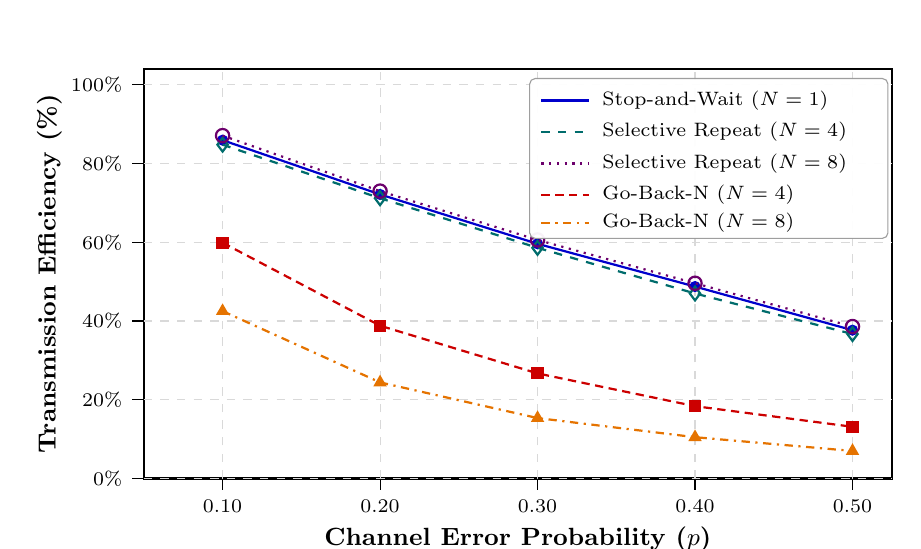
\begin{tikzpicture}[font=\footnotesize]
        % --- GRID & AXIS BOX ---
        \draw[thick] (1.0, 0) rectangle (10.5, 5.2);

        % Horizontal grid lines & Y ticks
        \foreach \y/\val in {0/0, 1/20, 2/40, 3/60, 4/80, 5/100} {
            \draw[dashed, black!15] (1.0, \y) -- (10.5, \y);
            \draw (1.0, \y) -- (0.85, \y) node[left, font=\scriptsize] {\val\%};
        }

        % Vertical grid lines & X ticks
        \foreach \x/\val in {2.0/0.10, 4.0/0.20, 6.0/0.30, 8.0/0.40, 10.0/0.50} {
            \draw[dashed, black!15] (\x, 0) -- (\x, 5.2);
            \draw (\x, 0) -- (\x, -0.15) node[below, font=\scriptsize] {\val};
        }

        % Axis Labels
        \node[below=14pt, font=\small\bfseries] at (5.75, 0) {Channel Error Probability (\(p\))};
        \node[font=\small\bfseries, rotate=90] at (-0.2, 2.6) {Transmission Efficiency (\%)};

        % --- PLOTS ---
        % 1. Stop-and-Wait (blue solid, filled circle)
        \draw[thick, blue!80!black, mark=*, mark size=1.6pt] plot coordinates {
            (2.0, 4.297) (4.0, 3.608) (6.0, 2.981) (8.0, 2.438) (10.0, 1.884)
        };

        % 2. Selective Repeat N=4 (teal dashed, open diamond, slight visual offset for visibility)
        \draw[thick, teal!85!black, dashed, mark=diamond, mark size=2.5pt, mark options={solid, thick}] plot coordinates {
            (2.0, 4.240) (4.0, 3.560) (6.0, 2.930) (8.0, 2.350) (10.0, 1.835)
        };

        % 3. Selective Repeat N=8 (violet dotted, open circle, slight visual offset for visibility)
        \draw[thick, violet!85!black, dotted, mark=o, mark size=2.4pt, mark options={solid, thick}] plot coordinates {
            (2.0, 4.355) (4.0, 3.650) (6.0, 3.030) (8.0, 2.480) (10.0, 1.930)
        };

        % 4. Go-Back-N N=4 (red densely dashed, square)
        \draw[thick, red!80!black, densely dashed, mark=square*, mark size=1.8pt, mark options={solid}] plot coordinates {
            (2.0, 2.995) (4.0, 1.941) (6.0, 1.335) (8.0, 0.919) (10.0, 0.657)
        };

        % 5. Go-Back-N N=8 (orange dashdotted, triangle)
        \draw[thick, orange!90!black, dashdotted, mark=triangle*, mark size=2.0pt, mark options={solid}] plot coordinates {
            (2.0, 2.126) (4.0, 1.221) (6.0, 0.768) (8.0, 0.525) (10.0, 0.350)
        };

        % --- LEGEND BOX (Top-Right) ---
        \draw[fill=white, draw=black!40, rounded corners=2pt, opacity=0.95] (5.9, 3.05) rectangle (10.45, 5.08);

        \begin{scope}[font=\scriptsize]
            % Entry 1: S&W
            \draw[thick, blue!80!black, mark=*, mark size=1.5pt] (6.05, 4.8) -- (6.65, 4.8);
            \node[right] at (6.7, 4.8) {Stop-and-Wait (\(N=1\))};

            % Entry 2: SR N=4
            \draw[thick, teal!85!black, dashed, mark=diamond, mark size=2.2pt, mark options={solid, thick}] (6.05, 4.4) -- (6.65, 4.4);
            \node[right] at (6.7, 4.4) {Selective Repeat (\(N=4\))};

            % Entry 3: SR N=8
            \draw[thick, violet!85!black, dotted, mark=o, mark size=2.1pt, mark options={solid, thick}] (6.05, 4.0) -- (6.65, 4.0);
            \node[right] at (6.7, 4.0) {Selective Repeat (\(N=8\))};

            % Entry 4: GBN N=4
            \draw[thick, red!80!black, densely dashed, mark=square*, mark size=1.5pt, mark options={solid}] (6.05, 3.6) -- (6.65, 3.6);
            \node[right] at (6.7, 3.6) {Go-Back-N (\(N=4\))};

            % Entry 5: GBN N=8
            \draw[thick, orange!90!black, dashdotted, mark=triangle*, mark size=1.6pt, mark options={solid}] (6.05, 3.25) -- (6.65, 3.25);
            \node[right] at (6.7, 3.25) {Go-Back-N (\(N=8\))};
        \end{scope}

    \end{tikzpicture}
    \caption{Protocol transmission efficiency versus channel error probability \(p\) (\(10{,}000\) frame trials; S\&W, SR \(N=4\), and SR \(N=8\) follow the theoretical \(1-p\) trajectory).}
    \label{fig:efficiency_plot}
\end{figure}

% =========================================================================
% SECTION 7: LIVE EXECUTION TRACES AND SOCKET TRANSCRIPTS
% =========================================================================
\section{Live Execution Traces and Socket Transcripts}

The compiled binaries \texttt{receiver.exe} and \texttt{sender.exe} were executed natively over TCP loopback (\texttt{127.0.0.1:5000}) with \texttt{input.txt}. The captured transcripts illustrate the distinctive protocol dynamics.

\subsection{Trace 1: Stop-and-Wait ARQ Error Injection and Retransmission}

Listing~\ref{lst:saw_trace} demonstrates how a single-bit error injected during the transmission of sequence 0 corrupts the frame, causes the receiver to withhold its ACK, triggers a 1500 ms sender timeout, and culminates in a successful retransmission.

\begin{lstlisting}[style=hexstyle, caption={Live socket execution trace: Stop-and-Wait ARQ error recovery.}, label={lst:saw_trace}]
============================================
FRAME SEQUENCE NUMBER: 0
Error Detection: CRC-32 | Channel Error Simulation: ENABLED
Original Payload (Text): "The morning sun begins to warm the quiet park."
Original FCS: 0x3DE9981E

Single Bit Error Injected.
Channel result: ERROR INJECTED.
Transmitted Frame Payload: "Th% morning sun begins to warm the quiet park."
Frame sequence 0 sent (65 bytes).
ACK timeout for sequence 0.

Timeout/no valid ACK. Retransmission 1 of 5 for sequence 0.
Channel result: NO ERROR on this attempt.
Transmitted Frame Payload: "The morning sun begins to warm the quiet park."
Frame sequence 0 sent (65 bytes).
ACK received for sequence 0.
Frame successfully acknowledged.
\end{lstlisting}

\subsection{Trace 2: Go-Back-N Window Retransmission Multiplication}

Listing~\ref{lst:gbn_trace} captures the Go-Back-N window behavior (\(N=4\)). Frame 1 encounters a bit error. The receiver silently drops frame 1 and subsequent out-of-order frames 2, 3, and 4. Upon timeout on frame 1, the sender retransmits the \textbf{entire window} (\([1..4]\)).

\begin{lstlisting}[style=hexstyle, caption={Live socket execution trace: Go-Back-N ARQ full-window retransmission.}, label={lst:gbn_trace}]
Frame sequence 0 sent (65 bytes) -> Cumulative ACK received for sequence 0.
Frame sequence 1 sent (65 bytes) -> [ERROR INJECTED: Bit flip in payload]
Frame sequence 2 sent (65 bytes) -> [Receiver discards: Out-of-order]
Frame sequence 3 sent (65 bytes) -> [Receiver discards: Out-of-order]
Frame sequence 4 sent (65 bytes) -> [Receiver discards: Out-of-order]

Timeout waiting for ACK of sequence 1.
Go-Back-N Retransmission 1 of 5 for window [1..4].
  Retransmitting sequence 1 -> Frame sequence 1 sent (65 bytes).
  Retransmitting sequence 2 -> Frame sequence 2 sent (65 bytes).
  Retransmitting sequence 3 -> Frame sequence 3 sent (65 bytes).
  Retransmitting sequence 4 -> Frame sequence 4 sent (65 bytes).
Cumulative ACK received for sequence 4 (acknowledges frames 1 through 4).
Window slides to base 5.
\end{lstlisting}

\subsection{Trace 3: Selective Repeat Out-of-Order Buffering}

Listing~\ref{lst:sr_trace} illustrates Selective Repeat (\(N=4\)). Frame 3 is corrupted. Correctly received frames 4 and 5 are buffered in the receiver's window and independently acknowledged. Upon timeout, \textbf{only} frame 3 is retransmitted, after which all buffered frames are delivered to the application in sorted order.

\begin{lstlisting}[style=hexstyle, caption={Live socket execution trace: Selective Repeat selective retransmission.}, label={lst:sr_trace}]
Frame sequence 3 sent (65 bytes) -> [ERROR INJECTED: Corrupted, discarded]
Frame sequence 4 sent (65 bytes) -> Receiver buffers frame 4; sends ACK 4.
Selective ACK received for sequence 4 (Window base remains at 3).
Frame sequence 5 sent (65 bytes) -> Receiver buffers frame 5; sends ACK 5.
Selective ACK received for sequence 5 (Window base remains at 3).

Timeout for sequence 3. Selectively retransmitting unacknowledged frames.
  Selectively retransmitting sequence 3 -> Frame sequence 3 sent (65 bytes).
Selective ACK received for sequence 3.
Window slides past acknowledged sequence 3.
Delivering sorted frame sequence 3 ("Please remember to close the door right away!!")
Delivering sorted frame sequence 4 ("The children love playing in the green grass!!")
Delivering sorted frame sequence 5 ("He always enjoys a hot cup of tea in morning!!")
All buffered frames delivered in sorted order.
\end{lstlisting}

% =========================================================================
% SECTION 8: ANALYSIS AND DISCUSSION
% =========================================================================
\section{Analysis and Discussion}

\subsection{Comparative Analysis across Test Cases}

\begin{enumerate}
    \item \textbf{Propagation Delay Sensitivity (\(a = T_{\text{prop}} / T_{\text{tx}}\)):} In Test Case 1, as propagation delay increased from \(5\text{ ms}\) to \(50\text{ ms}\), the Round-Trip Time escalated from \(10.1\text{ ms}\) to \(100.1\text{ ms}\). In Stop-and-Wait, the sender remains completely idle during this interval. With \(T_{\text{prop}} = 50\text{ ms}\) and \(T_{\text{tx}} = 0.052\text{ ms}\), \(a \approx 961\), collapsing Stop-and-Wait channel utilization to \(\eta \approx 0.05\%\). Conversely, pipelined protocols (GBN and SR) fill the pipeline with \(N\) frames, scaling throughput by a factor of \(N\).

    \item \textbf{Impact of Error Probability on Retransmission Multiplier:} Test Case 3 empirically highlights the fundamental limitation of Go-Back-N. When an error occurs at \(p = 0.50\), GBN (\(N=4\)) generated \textbf{\(66{,}104\) retransmissions} to deliver \(10{,}000\) frames, causing its transmission efficiency to plunge to \(13.14\%\). In contrast, Selective Repeat (\(N=4\)) generated only \textbf{\(16{,}816\) retransmissions}, matching the transmission efficiency of Stop-and-Wait (\(37.29\%\) vs.\ \(37.67\%\)) while retaining the throughput benefits of sliding-window pipelining.

    \item \textbf{Receiver Complexity vs. Channel Quality Trade-Off:} Go-Back-N requires minimal receiver memory (buffer size = 1) and no sorting logic, making it ideal for resource-constrained embedded systems on low-error channels (\(p < 0.01\)). However, on noisy channels (\(p > 0.10\)), Selective Repeat's memory overhead (buffer size = \(N\)) is heavily justified by its superior bandwidth conservation.
\end{enumerate}

\subsection{Known Limitations and Practical Enhancements}

\begin{itemize}
    \item \textbf{Negative Acknowledgments (NAK):} The current implementation relies strictly on sender timeout expiration to detect frame loss. Integrating NAK frames upon detecting out-of-order sequence arrival would trigger immediate retransmissions, eliminating idle timeout delays.
    \item \textbf{Bidirectional Piggybacking:} Currently, data frames and ACK frames travel over separate application messages. In production protocols, reverse-direction data frames embed acknowledgment sequence numbers inside their headers (piggybacking), drastically reducing channel overhead.
    \item \textbf{Dynamic Jacobson-Karn RTT Estimation:} The evaluated socket implementation utilized a fixed 1500 ms timeout. Production transport layers track smoothed round-trip time (\(SRTT\)) and variance (\(RTTVAR\)):
    \begin{align}
        SRTT &\leftarrow (1 - \alpha) \cdot SRTT + \alpha \cdot RTT_{\text{sample}} \\
        RTTVAR &\leftarrow (1 - \beta) \cdot RTTVAR + \beta \cdot |SRTT - RTT_{\text{sample}}| \\
        RTO &= SRTT + 4 \cdot RTTVAR
    \end{align}
    Implementing adaptive timeout estimation prevents premature timeouts caused by network jitter.
\end{itemize}

% =========================================================================
% SECTION 9: COMMENTS AND LEARNING EVALUATION
% =========================================================================
\section{Comments and Learning Evaluation}

\subsection{Evaluation of the Lab Assignment}

This lab assignment provided invaluable practical insight into the foundational mechanisms that underpin reliable data communications. Designing and implementing Stop-and-Wait, Go-Back-N, and Selective Repeat from the ground up illuminated the complex interplay between framing, serialization, asynchronous socket I/O, timer management, and state machine transitions.

\subsection{What I Learned}

\begin{itemize}
    \item \textbf{Sliding Window Mechanics:} Understanding how window boundaries (\texttt{base}, \texttt{nextSeq}) slide dynamically upon receiving cumulative versus independent acknowledgments.
    \item \textbf{Receiver Reassembly:} Managing out-of-order buffers in Selective Repeat and ensuring that frames are delivered to the application layer in strict sequential order.
    \item \textbf{Concurrency and Socket Timeouts:} Configuring non-blocking or timed socket operations (\texttt{SO\_RCVTIMEO}) across platforms (Winsock2 on Windows vs. BSD sockets on Linux) to prevent indefinite application hangs.
    \item \textbf{Empirical Protocol Benchmarking:} Quantifying the exact performance penalties of retransmission multiplication in GBN versus selective buffering in SR across diverse channel conditions.
\end{itemize}

\subsection{Difficulty Assessment}

The assignment was moderately challenging but highly rewarding:
\begin{itemize}
    \item \textbf{Why it was challenging:} Handling timer expirations within a pipelined socket loop without multi-threading or external event libraries required careful state tracking. Implementing the circular sequence number logic and avoiding sequence ambiguity demanded rigorous validation.
    \item \textbf{Why it was manageable:} Building directly upon the framing, checksum, and CRC modules established in Assignment 1 provided a robust foundation, allowing the focus to remain on flow control algorithms.
\end{itemize}

\subsection{Suggested Improvements}

\begin{enumerate}
    \item Provide an explicit software channel emulation interface capable of injecting configurable latency jitter and random packet dropping at the transport level to simulate wide-area internet connections.
    \item Extend the assignment to incorporate Negative Acknowledgments (NAK) and selective acknowledgment (SACK) blocks similar to RFC 2018 in modern TCP.
\end{enumerate}

% =========================================================================
% SECTION 10: SOURCES USED
% =========================================================================
\section{Sources Used}

\begin{enumerate}
    \item Kurose, J. F., and Ross, K. W., \textit{Computer Networking: A Top-Down Approach}, 8th ed., Pearson, 2021.
    \item Tanenbaum, A. S., and Wetherall, D. J., \textit{Computer Networks}, 5th ed., Prentice Hall, 2011.
    \item Stallings, W., \textit{Data and Computer Communications}, 10th ed., Pearson, 2014.
    \item IEEE Standard for Ethernet (IEEE Std 802.3-2022) and POSIX / BSD Socket API Reference Documentation.
    \item AI Assistance and Antigravity: Artificial intelligence assistance (Gemini) was utilized for statistical aggregation, benchmarking script construction, and generating native TikZ visualization code. The Antigravity development environment was used to run live socket test executions, profile empirical performance metrics, and format the comprehensive \LaTeX{} report.
\end{enumerate}

\end{document}
